%%
%% Template intro.tex
%%

\chapter{Background}
\label{cha:back}

In the following, we define the source of our data set, notation used throughout this thesis, our choice of prediction algorithms and 
our testing appraoch and methodology.

\section{Facebook}
\label{sec:data}

Facebook is the largest and most active social media service in the world. Facebook users can create a profile containing personal preferences 
and have friendships and interactions between other users. These interactions can also be liked or commented on by other users.

discuss feed time for facebook

need to show all different ways to interact

\section{LinkR}
\label{sec:linkr}

NICTA developed a Facebook app named LinkR \footnote{The main developer of the LinkR
Facebook App is Khoi-Nguyen Tran, a PhD student at the Australian
National University.  Khoi-Nguyen wrote the user interface and database
crawling code for LinkR.} 
which would make recommendations to app users and record whether or not the user liked the item.

The dataset includes information about each app user as well as a subset of available data about their friends.

The LinkR Facebook app was used to collect information about users, their interactions and preferences. The data set contains information about app users as 
well as a sub-set of visible information about their friends. The app tracked and stored information for over 100 app users and their 39,000+ friends.

The four main interactions between users are posts (posting an element on a friends' wall), tags (being mentioned in a friends post or comment), 
comments (written data on a post) and likes (clicking a like button if a user likes a post or comment). The table below outlines data collected during 
app trials.
 
The table below summarises the data collected from both app users and their friends.

\begin{table}[!htbp]
\centering
	\begin{tabular}{|l|r|r|r|r|} % cols: (left, center, right)
		\hline
		\textbf{App Users} & \textbf{Posts} & \textbf{Tags} & \textbf{Comments} & \textbf{Likes}  \\ \hline
		\textbf{Wall} & 27,955 & 5,256 & 15,121 & 11,033 \\ \hline
		\textbf{Link} & 3,974 & - & 5,757 & 4,279 \\ \hline
		\textbf{Photo} & 4,147 & 22,633 & 8,677 & 5,938 \\ \hline
		\textbf{Video} & 211 & 2,105 & 1,687 & 710 \\ \hline
		 \hline
		\textbf{App Users and Friends} & \textbf{Posts} & \textbf{Tags} & \textbf{Comments} & \textbf{Likes}  \\ \hline
		\textbf{Wall} & 3,384,740 & 912,687 & 2,152,321 & 1,555,225 \\ \hline
		\textbf{Link} & 514,475 & - & 693,930 & 666,631 \\ \hline
		\textbf{Photo} & 1,098,679 & 8,407,822 & 2,978,635 & 1,960,138 \\ \hline
		\textbf{Video} & 56,241 & 858,054 & 463,401 & 308,763 \\ \hline
	\end{tabular}
	\caption{Data records for interactions between users. Rows are the type of interaction, columns are the context.}
	\label{tab:revpol}
\end{table}

Pertanent user data which is collected by the LinkR app includes:
\begin{itemize}
\item Gender
\item Age
\item Hometown
\item Locale
\item Group Memberships
\item Page Likes
\item Favourite Activities
\item Favourite Books
\item Favourite Athletes
\item Favourite Teams
\item Inspirational People
\item Interests
\item Favourite Movies
\item Favourite Music
\item Favourite Sports
\item Favourite Television Shows
\item School Information
\item Work Information
\item Messages data
\end{itemize}

\section{Notation}
\label{sec:notation}

The mathematical notation used by our classifiers during this thesis are outlined below.


define k for exposire
alters

\begin{figure}[h]
	\begin{center}
		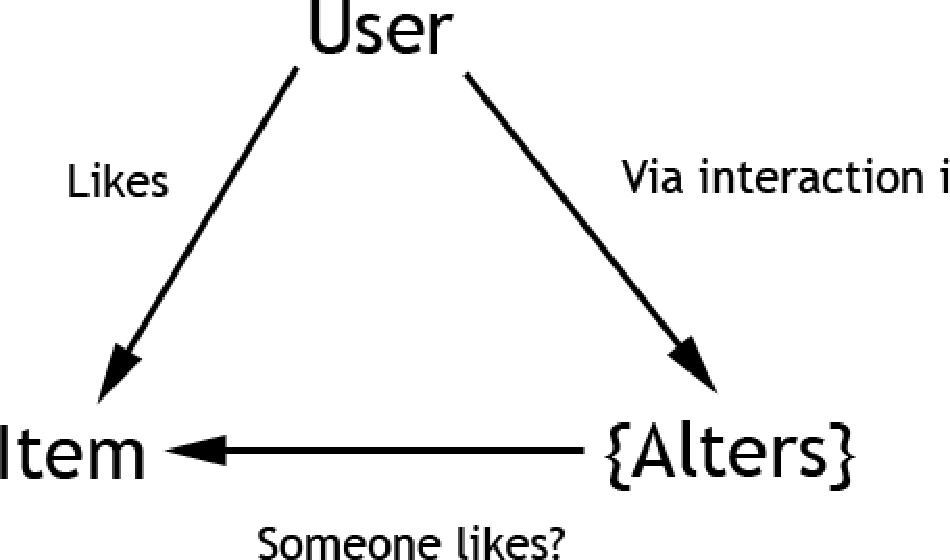
\includegraphics[scale=0.60]{imgs/alters.pdf}
		\caption{Predictors paradigm}
	\end{center}
\end{figure}

\begin{itemize}
\item $N$ users. 
\item $M$ items.
\item A user feature set $F$ of size $i$.
\item A dataset $D$ comprised of $D = \{(n,m,f_i) \to y\}$ with the binary response $y \in \{0,1\}$ where $0$ represents a dislike and $1$ 
represents a like.
\end{itemize}

\section{Feature Sets}
\label{sec:features}

Need to discuss different feature sets

The feature sets in $x$ can be any of the following, which are discussed further in :::

\begin{itemize}
\item Interactions
\item Demographics
\item Traits
\item Groups
\item Pages
\item Outgoing Messages
\item Incoming Messages
\end{itemize}

\section{Previous Work}
\label{sec:pw}

While many Facebook users have a friend count which is close to the human real word limit, known as the Dunbar number ~\cite{hill2003social},
this work shows that user interactions are focused on a much smaller subset of their friends.

\cite{backstrom2011center} studied two types of user uses of Facebook, explicit communication interaction and viewing attention. Communication 
is focused on a limited subset of friends whilst viewing attention is dispersed among a much larger set. This supports the approach of testing
a wide array of user interactiuons and preferences, as each users preferences are driven by where their attention is focused.

\subsection{Content Based Filtering}
\label{sec:cbf}

Content based filtering (CBF) ~\cite{newsweeder} is an extension of the technique of Collaborative filtering (CF) ~\cite{collab_filtering} 
which predicts whether a user will like an item via information about that users' prefererences as well as that of other users, CBF extends 
this approach by generalising from the item features which the user has explicitly liked or disliked.

Based on previous user trials ~\cite{joseph} Social Matchbox was the best performing algorithm in live user trials, gaining more likes then
dislikes and hence will be the base line comparator used in this thesis.

\section{Classification Algorithms}
\label{sec:meth}

This analysis makes use of the results from a number of different classification algorithms which are outlined below.

\subsection{Constant}
\label{sec:const}

The constant predictor returns a constant result irrespective of the feature vectors selected from above. The most common result in our data
set is $False$ and hence the $False$ predictor is displayed in our analysis.

\subsection{Social Match Box}
\label{sec:sr}

Social Matchbox uses the Social Regularization method to incorporate the social in-formation of the Facebook data. ~\cite{joseph}

What this objective component does is constrain users with a high similarity rating to have the same values in the latent feature space. 
This models the assumption that users who are similar socially should also have similar preferences for items.

This method is an extension of existing SCF techniques~\cite{lla,socinf} that constrain the latent space to enforce users 
to have similar preferences latent representations when they interact heavily. Like Matchbox which extends regular matrix factorization
methods by making use of user and link features, our extension to the Social Regularization method incorporates user features to learn
similarities between users in the latent space.


\subsection{Naive Bayes}
\label{sec:nb}

\emph{Naive Bayes} (NB) is a basic predictor which involves applying Bayes' theorem using independence assumptions between each feature in $x$.

The NB implementation used during this thesis is an implementation previously devised by \emph{Scott Sanner} \cite{scott}.

\subsection{Logistic Regression}
\label{sec:lr}

\emph{Logistic Regression} (LR) predicts the odds of being either a like or a dislike by converting a dependent variable and one or more continuous 
independent variable(s) into probabability odds.

The LR implementation used during this thesis is \emph{LingPipe} \cite{lin}.

\subsection{Support Vector Machine}
\label{sec:svm}

The \emph{Support Vector Machine} (SVM) is a supervised learning machine based on a set of basis functions which help construct a separating 
hyperplane between the data points. Training involves buidling the relevant hyperplanes which can then be used for testing. Each data point is
classified depending on which side of the hyperplane it falls.

The SVM implementation used during this thesis is \emph{SVMLibLinear} \cite{cjlin}.

\section{Training and Testing}
\label{sec:tt}

All evaluation is done using 10 fold cross validation wherein the data is partitioned into 10 complimentary subsets, each subset is composed 
of two separate parts one section is used for training $(80\%)$ and the other $(20\%)$ is used for testing. This is performed on 10 distinct 
subsets and the results are averaged across each fold.

"has been shown that positive social annotations on search items adds perceived utiltiy to the worth of a result, particularly with close social
connections"
~\cite{pantel}

accuracy and exposure curve

all graphs accuracy

However, if we use only a subset of the data, holding out on only elements which have at least k likes amoung the group of alters 
we can compare using these exposure curves  which can provide some indicator of a users exposure to a liked item.

\section{Evaluation Metrics}
\label{sec:notation}

When evaluating the success of each method at correctly predicting the classification, the following metrics will be used.

\begin{itemize}
\item A \emph{true positive} prediction refers to when the classifier correctly identifies the class as true. 
\item A \emph{false positive} occurs when the prediction is true, but the true class was false. 
\item A \emph{false negative} occurs when the prediction is false but the actual class is true.
\end{itemize}

Accuracy relates to the closeness to the true value. In the context of our results, the accuracy refers to the number of correct classifications 
divided by the size of the data set.

\[ \text{accuracy} = \frac{\text{number of correct classifications}}{\text{size of the test data set}}\]

Precision relates to the number of retrieved predictions which are relevant. In the context of our results, the precision refers to the number of true positive predictions 
divided by the sum of the true positive and false positive predictions.

\[ \text{precision} = \frac{\text{number of true positives}}{\text{number of true positives + number of false positives}}\]

Recall refers to the number of relevant predictions that are retrieved. In the context of our results, recall refers to the number of true positive predictions 
divided by the sum of the true positive and false negative predicitons.

\[ \text{recall} = \frac{\text{number of true positives}}{\text{number of true positives + number of false negatives}}\]

The f-score combines and balances both precision and recall and is refered to as the weighted average of both precision and recall. 

\[ \text{f-score} = 2 \times \frac{\text{precision} \times \text{recall}}{\text{precision} + \text{recall}}\]

The main metric we use for analysis in this thesis is accuracy.

%%% Local Variables: 
%%% mode: latex
%%% TeX-master: "thesis"
%%% End: 
